\chapter{Introduction and Motivation}
% Should I add a section to mention my professional background that's relevant and which inspired my PhD?
I have been actively involved in testing mobile apps professionally and as a volunteer since 2006. I, together with a plethora of others have also researched testing of mobile apps applying a vast range of ideas and approaches together with seeking ways to measure the effectiveness of these approaches and ideas. Ultimately, the vast majority of mobile apps are intended to be used by end-users rather than as research tools. Therefore I reasoned a useful approach might be to measure the effectiveness of testing through information pertaining to their use of the mobile apps. This is not intended to negate other measures, and some aspects of testing may be hard to measure or somewhat irrelevant to measure using my proposed approach, for instance testing for security vulnerabilities might be measured more effectively using other approaches and techniques.

Mobile apps are ubiquitous and range from trivial entertainment to mission-critical and even life-critical. Users want to trust the apps work well and do what they are supposed to, without misbehaving, cheating, or failing i.e. users need trustworthy mobile apps. My research aims to explore the potential of two complementary sources of analytic data: data collected at a device or system level by the Android platform (in conjunction with Google Mobile Services), and data collected by one or more software libraries optionally incorporated into the app itself. 

The work focuses on the Android platform and Android apps:
\begin{itemize}
    \item Android is the largest mobile platform and ecosystem globally.
    \item It is the most researched mobile platform in terms of researchers and publications. Much of the software, including test automation, is open sourced.
    \item Android Vitals is an excellent example of a platform-wide tool aimed at helping developers learn about their apps and how they behave. Usage by the crowd is gathered by the platform\todo{Mention the 'Machine - Platform - Crowd' book once I have read it.}
    \item The problem space is far larger and more extensive than the iOS ecosystem.
    \item The author actively works on various Android apps and obtained greater support from developers of Android apps than for other platforms.
\end{itemize}

\section{"The proof of the pudding is in the eating"}
Whatever other testing is done, or left undone, for Android apps they are ultimately tested in use on end-user devices and by end-users. These tests are often implicit and \textit{ad-hoc}. Clues of the results may be found in various places, in ratings and reviews, in uninstalls, in usage (and disuse), and through reported failures. Extensive research has been carried out related to ratings and reviews, these will be covered later in this thesis. % I could have a go at expanding this section here to summarise the broad themes people have researched. 
These include analysing reviews for bug reports, % add ref
prioritising testing based on the devices game players used to \textit{write} their reviews on (on the basis they're probably writing the review from the same device that they played the game on), % add ref
and automatically creating tests based on the content of reviews. % add ref
Blah has compared ratings with assessments of the quality of the code of mobile apps. % add ref

Perhaps unsurprisingly the vast majority of research is where it's both easier and popular to do - for Android apps and the Android+Google ecosystems. [Or should I aim to be more explicit and explain the reasons why researchers seem to focus on Android e.g. opensource, availability of software tools, most researchers are working with Western-oriented Google Play apps (rather than Chinese app stores, etc).]

Several app stores \iffalse I think only a few, Android, Apple, and perhaps some in China \fi include software that runs on end-user devices that can collect various run-time data; users opt-in to providing the data to the app store, and in turn the app store chooses how much data to provide to the development teams. For Android, Google provides the Google Play Console that incorporates tools, known as Android Vitals % add refs
, to enable development teams to learn about various aspects of their Android apps, including problems and failures. Android Vitals seemed to offer tools that might help measure the effectiveness of past testing of that Android app. \hyperlink{android_vitals}{Android Vitals} will be introduced further in this introduction and this approach will be expanded later in a subsequent chapter. % TODO add text and link to the chapter

Explicit testing in enclosed environments (e.g. a team, organisation, and to a lesser extent alpha testing) is not likely to scale to the any of the dimensions of how the app will be used; \textit{perhaps there are a few slivers where the testing would scale for a few apps (e.g. one written solely for a few users in tightly controlled conditions), for the purposes of my research I will not focus on these unusual cases}. 

As a practical example, the range of Android devices far exceeds the number used by most teams to test their app. An organisation,  OpenSignal, produced a series of annual reports for several years where they analysed various aspects of the user base of mobile apps they provided free of charge for end users to measure their mobile device's connectivity. They discovered their Android app was used on over 24,000 distinct device models, % add citation to the report
they graphed the distribution as shown in figure \ref{fig:opensignal_devices}. At the time, their app was used most on a Samsung Galaxy S III. Perhaps the team might be wise to prioritise testing on the same device model? If the team wanted to test on more than one device model, which would they pick? and so on and so on. However, regardless of how many device models they test on, and how they decide which models to use, they are extremely unlikely to test on even 1\% of the device models so the behavior of their apps across the set of devices their users use is not well known despite diligent testing locally.

TBC Discuss whether testing on a subset of devices is adequate. Use the example of selecting representative devices using OpenSignal's Manufacturer Graph as one source.

\begin{figure}
    \centering
    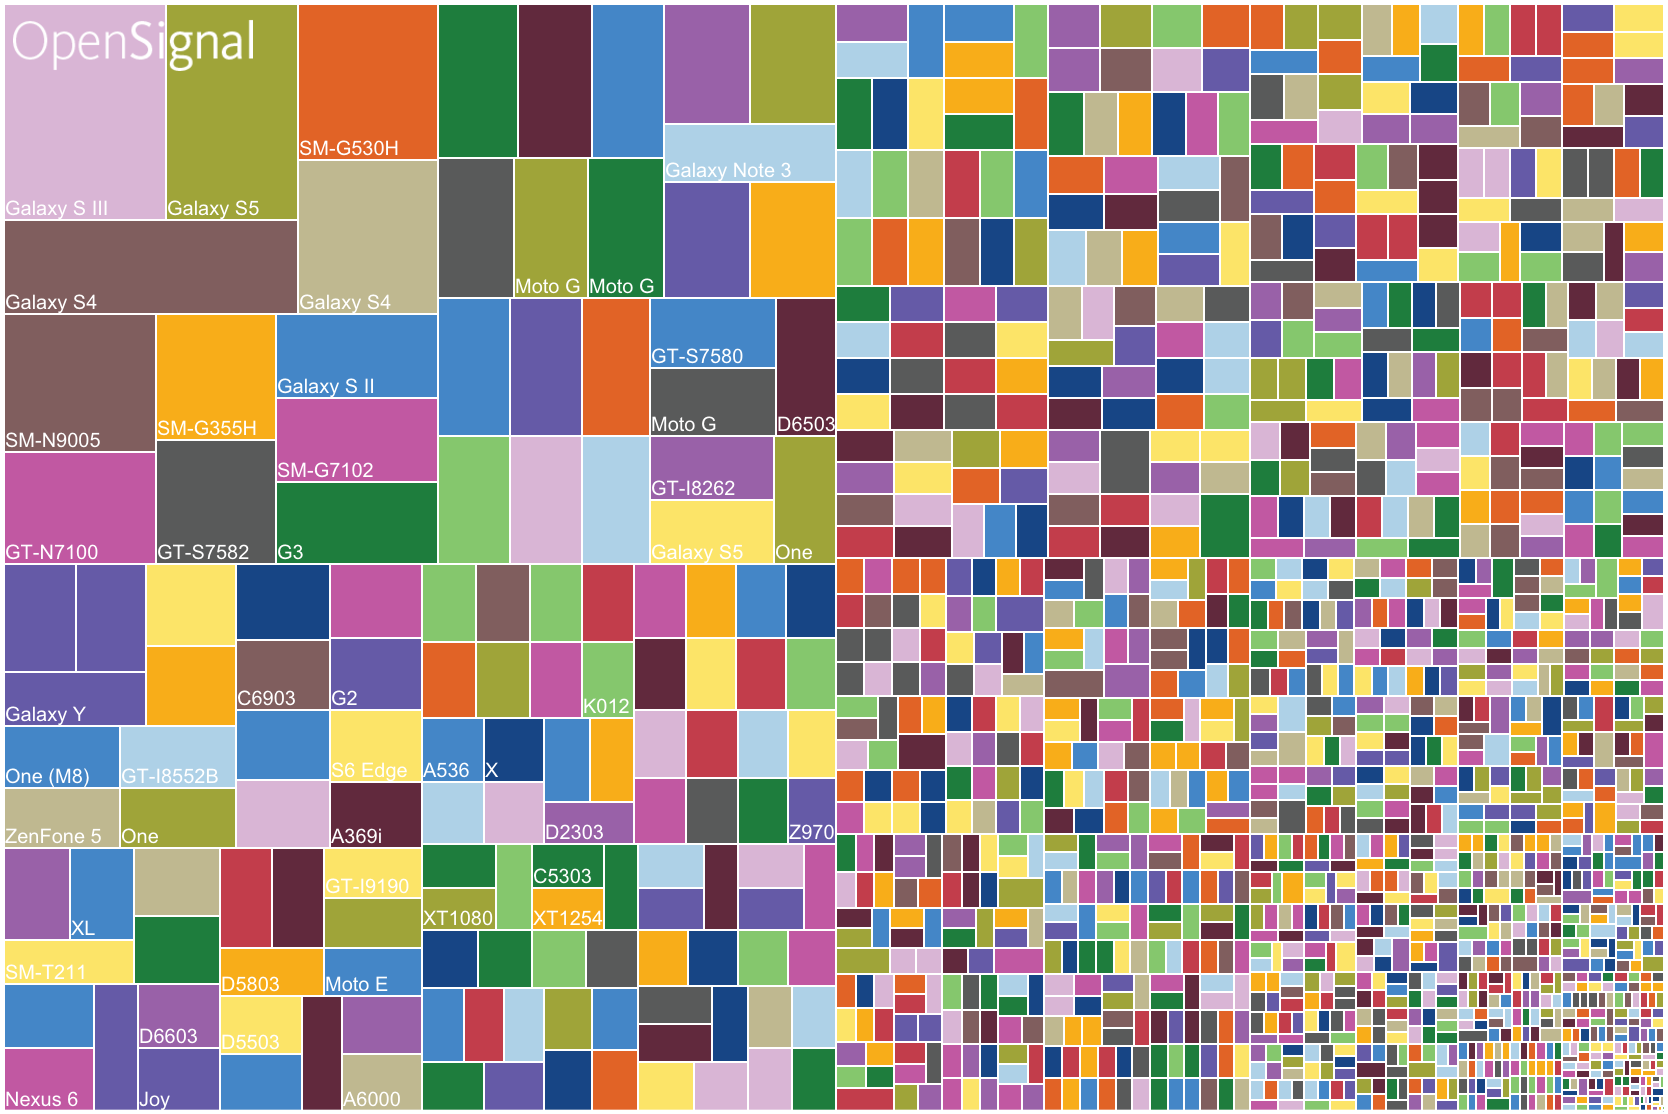
\includegraphics[angle=90,origin=c, width=\textwidth,height=\textheight,keepaspectratio]{images/opensignal-android-devices-matrix.png}
    \caption{OpenSignal Android Devices}
    \label{fig:opensignal_devices}
\end{figure}
% How to rotate a figure https://latex.org/forum/viewtopic.php?t=9323
% Ways to shrink the image to fit a single page https://tex.stackexchange.com/questions/32886/how-to-fit-a-large-figure-to-page

Fan-out ratios for popular apps can be in their tens of millions, between the people involved in creating the app and those who use them. An extreme example is WhatsApp who had 50 engineers supporting a user-base of 900m, a fan-out ratio of 1:18,000,000 (1 engineer for every 18m users)\footnote{\url{https://web.archive.org/web/20171018201359/https://www.wired.com/2015/09/whatsapp-serves-900-million-users-50-engineers/}}. As the fan-out ratio increases so can the communications challenges between developers and their users. Logging and analytics may help make communication between the app and the developer scale and be viable. Analytics may help interpret firehoses of data into insights. 

Testing is not the only way to assess software quality, there are other ways such as using and applying static analysis tools, code reviews, popularity, and so on. Nonetheless the concept of testing software, including mobile apps, has become established \textit{even by those who barely test their apps}.

\section{Components of Software Quality}

\begin{itemize}
    \item What is quality? According to whom? 
    \item Different perceptions of quality.
\end{itemize}

\begin{figure}
    \centering
    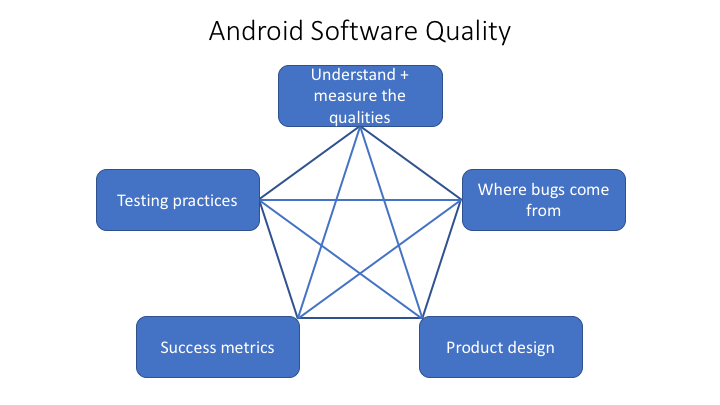
\includegraphics[width=\columnwidth]{images/Android_Software_Quality.png}
    \caption{Android Software Quality}
    \label{fig:android_software_quality}
\end{figure}

Figure \ref{fig:android_software_quality} illustrates five interrelated factors that seem to underpin software quality for Android apps. There may be additional factors, for now these have proven useful to help structure my research.

\subsection{Understand and Measure Qualities}
Much rests on the understanding and interpretation of what quality is or what qualities are as pertains Android apps. It seems safe to state that no single, agreed-upon definition or understanding of software quality. This lack of agreement or coherence may fragment our work and research, nonetheless we have found ways to measure and address several aspects of software quality through our research.

Software tools can help measure facets of quality. So can user ratings. \textbf{\textit{One of our challenges as researchers is to decide on KPIs we want to track as we change from where we are to where we want to reach...}}

\begin{table}[]
    \centering
    \footnotesize
    \begin{tabular}{l|l|l}
        Approach     & Source & Measures \\
        \hline
        Heatmapping  & Digital & User interactions with GUI \\
        User Ratings & Analogue & Subjective score of an app \\
        User Reviews & Analogue & Subjective written feedback \\
        Android Vitals & Digital & "Stability" measures of an app \\
        Activity & Digital & Installs, sessions, usage, etc. \\
        Mobile Analytics & Digital & Device details \& settings, app specific usage data, etc. \\
        Crash recording & Digital & Exceptions 
    \end{tabular}
    \caption{Possible measurements of quality}
    \label{tab:quality_measurements}
\end{table}

In Table \ref{tab:quality_measurements} analogue indicates the source of the data is from users - user-generated assessments. Digital sources are collected programmatically, either because the developers have incorporated particular software to do so, or because the operating system collects the data.

\subsection{Success metrics}
Success factors for an app may affect the assessment of software quality and vice-versa, particularly in terms of relative importance. \textbf{We may use the success factors to interpret or weigh the KPIs.}

For instance, is activity a measure of success? (e.g. in terms of popularity, frequency and duration of use, etc.) Are the installs, active users, revenue, market penetration, influence, ratings, etc.? 

\subsection{Product Design}
This includes UI and UX design. Designing software to suit the user is likely to positively affect the perceived quality of the software. And better designs may lead to more usage, longer retention, more positive ratings and reviews, promotion of the app in the app store, etc.

Development practices, such as deciding whether to use a common codebase or custom codebases may also affect the product quality. Excess code is a burden, both in terms of maintainability and at run-time. \textit{Discuss the Kiwix custom app experience}.

\subsection{Where Bugs come from}

\subsection{Testing and Observability}
Testing is not the only way to assess software, we can also observe its behaviour in use. Figure \ref{fig:katrinaclokie_venndiagram_testing_and_observability_from_twitter} provides a friendly, visual introduction to possible overlap and what makes each distinct.

\begin{figure}
    \centering
    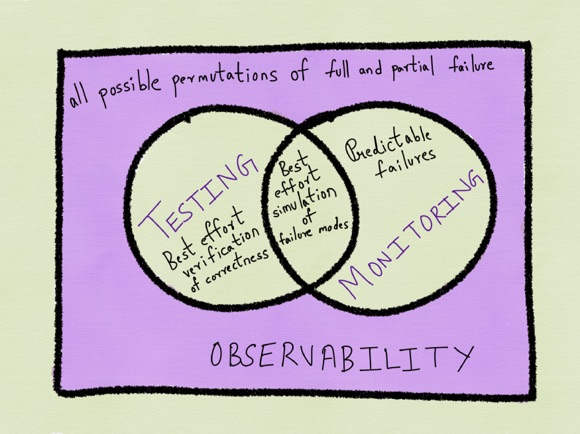
\includegraphics[width=\textwidth]{images/katrinaclokie_venndiagram_testing_and_observability_from_twitter.jpg}
    \caption{Katrina Clkie: Testing and Observability Venn Diagram}
    \small\textsuperscript{source:  \url{https://twitter.com/katrinaclokie/status/1189254727126659073/photo/1}}
    \label{fig:katrinaclokie_venndiagram_testing_and_observability_from_twitter}
\end{figure}
% Thanks to https://tex.stackexchange.com/questions/10181/using-footnote-in-a-figures-caption

Analytics tools can improve the observability of software's behaviour \emph{in use}. They may also provide feedback on aspects of the testing that has been performed on the releases that are currently in use.

Discuss DDP, confirmation of existing bugs (c.f. how Android Vitals and Pre-launch test results are automatically linked).

\subsection{Testing Practices}

\subsection{Related aspects}

Release practices: including when and how changes are applied and made available to users. 

\section{Core Concepts}
OK, to try and keep me on track, here's my precis of what I'm trying to do and evaluate...

\begin{itemize}
    \item Mobile apps are used globally, millions of people are involved in their ecosystems. These people, together with some 'users' actively test the apps.
    \item Testing is considered to be somewhere between desirable and essential. 
    \item Whether we realise it, or not, our testing isn't going to cover even everything we'd like to test. Also there's a point where it's not viable to try. 
    \item There are lots of approaches to testing mobile apps and various techniques.
    \item In practice, for most testers their perspectives are materially limited. There are various sources of data that may help them improve their testing if and when they use it. 
    \item Some of the data may already exist (even if they're not yet aware of it). In addition, additional data collection could be incorporated into the mobile app.
    \item The data may range from simple to complex. Similarly, the testing may range in complexity.
    \item There are other ways to do better testing and/or improve the quality of mobile apps. Does any of these obviate the value of using mobile analytics i.e. is there a better/easier/less-demanding/cheaper approach known to the community? 
    \item For mobile apps there are various practical considerations; these include data transmission and collection, privacy and sensitivity of what's collected, etc.
    \item There are also ethical and other concerns related to collecting and keeping data, concepts such as Datensparsamkeit\cite{fowler_datensparsamkeit_2013} (data minimisation) apply. Furthermore, investigating the relationship between the amount of data and its value and utility may help both researchers and practitioners. And establishing dynamic heuristics to govern what data to collect, transmit, and utilise may also reduce any data burden (the burden of collecting, transmitting, processing, safe-keeping, and storing data), see \hyperlink{dynamiclogging}{Dynamic Distributed Logging and Analytics}.
\end{itemize}

Android apps are ubiquitous and used by over a billion people globally.

%\initial{T}
Testing of mobile apps is particularly challenging. Many people and companies have tried to address some of these challenges\yijun{need to enumerate the challenges} and they continue to make progress in various ways using a rich variety of approaches. However, few appear to use usage data to inform their software testing which is the main focus of my research.\yijun{Would be good to find a citation for these statements, or add according to the author's own professional experience}

My work and research explores two complementary sources of digital data; the first is data collected by Google Play from users who have opted-in to providing failure data (including crashes and GUI freezes (known as Application Not Responding, or ANRs). The second uses mobile analytics which needs to be incorporated into mobile apps to provide a mix of predetermined and developer-added recording of additional events, etc.\yijun{need to justify why these two sources are chosen, for example, why not NPE null pointer exception bugs}\yijun{later needs to explain how these two complement each other}

These two sources of digital data may provide feedback on how well we developed and tested the app before, they may also lead to better testing and help with practical aspects such as reproducing failures so they are easier to test and assess.\yijun{Are these your own hypotheses? or would it worth to be stated explicitly as hypothesis to test in the study}

What we discover needs to be applied efficaciously in order to improve our practices and our products (mobile apps). Context often affects how the mobile apps behave and how they are perceived by users (who are one of the arbiters of the mobile apps) identifying the context that is relevant for the various purposes is a key consideration for my research and the approaches I have investigated. For instance, how and when is the version of Android relevant? and what do we lose if it is not available? \yijun{Somewhere to say why Android rather than iOS}

\textit{"He who gathers data related to others has responsibilities to uphold, ethically and often legally"} \footnote{along similar lines to \url{https://en.wikipedia.org/wiki/Quis\_custodiet\_ipsos\_custodes\%3F}}
so the research also explores aspects related to weighting the data we\yijun{We => need to distinguish researchers or developers} could collect with the risks, costs and responsibilities. A related consideration needs to be included where third-parties provide the services, software libraries, and control access to the data that has been collected. Their control may restrict our options, and also what are the considerations and implications if they wish to use the data that is collected?

The tools we use, and here Android Vitals and the various mobile analytics offerings, have a bearing on the quality of our work and the outcomes. Flaws, gaps, and other limitations in the tools may adversely affect our ability to improve our work and the software that \textit{we} create. From the outset I have been aware of inaccuracies in several of the tools, and during the research I have found and investigated how some of these tools perform. In doing so, bugs, inconsistencies, and improvements have been proposed to providers of tools, and to Google for Android Vitals in particular. We also wrote a scraper tool to be able to work with, analyse and process the data being presented by Android Vitals.

Testing of apps seldom stresses the apps with real-world imperfections; finding ways to test apps repeatably for at least the common issues (such as servers returning error codes, connections being broken, etc) should help increase the reliability and reduce the crash rate of the apps in real-world use. This paper helps set the scene for such testing. Combining their ideas with VanarSena (Microsoft's malicious test monkeys) may help us connect these approaches to testing with telemetric data from Google Play and Mobile Analytics.

Usage data comes from usage of mobile apps. I chose a family of Android apps from the Kiwix project as I am one of the volunteer contributors and have access to Google Play Console for the usage data it provides. Unfortunately from a research perspective, however materially for users of the software the Kiwix project does not actively collect any usage data from the apps. This led to various challenges for my research where I sought alternative projects who either already incorporate mobile analytics or would be willing to do so.

There are similarities between mobile analytics and logging by applications; the similarities indicate there was a great deal to learn from application logging and the tools related to processing these logs. Also, and particularly for very popular apps with millions of installs, dynamic logging can help reduce waste and resource consumption across the overall user population while also helping gather more detailed usage data for particular groups of users or patterns of activity.

My work fits in a broader context where there are many distinct approaches that offer the potential to improve the quality of mobile apps. For instance, static analysis tools can help catch some flaws in the application code and related resources (including text strings and image files, for instance). Orthogonally, many researchers have used ratings and reviews collected by app stores to help find flaws and improve testing of mobile apps.  Learning whether other approaches may find some of the flaws helps to position my work and research within the broader context, particularly as mobile analytics involves modifying the app's source code and/or the application binary.

We may also look further afield, for instance into AiOps, to explore whether there are useful parallels and connections between what they aim to achieve for their domain and I wish to achieve through my research. There is much to learn, and potential benefits from observing and learning about work beyond the albeit significant microcosm of mobile apps. My research has been positively influenced from research in logging, software analytics, and usage testing among others.

% https://www.microsoft.com/en-us/research/group/software-analytics/

For practical reasons the work is based on Android apps and tools for Android, I hope at least some of the work on mobile analytics will apply and be useful for developers of apps on iOS and other mobile platforms.

\textit{I have six honest serving men}

\textit{They taught me all I knew}

\textit{There names are What, and Where and When;}

\textit{and Why and How and Who.}

– Rudyard Kipling (1865-1936).

\textbf{Kipling on Software Testing} if we take Kipling's short \textit{Six Honest Serving Men} poem and adapt it to the domain of software testing we may be able to gain insights and identify possible sweet spots for various test techniques. Conversely, sometimes commonly practiced testing can be time-consuming yet not very productive.

\section{Software testing}
\subsection{Test Oracles}

\subsubsection{What is a test oracle?}
One factor to consider to assess whether something is a test oracle is the relative certainty or confidence that can be placed in the measure. An oracle \textit{is truth} a heuristic \textit{is fallible}. Both oracles and heuristics are used in software testing:

\subsubsection{Test heuristics}
provide examples of heuristics for testing mobile apps. COP FLUNG GUN and I SLICED UP FUN ...

\subsubsection{de-facto oracles}
\textit{We cannot prove the absence of bugs (TODO Find and add correct quote) we can detect their presence...}

de-facto defined: ....

de-facto test oracle: No reported crashes \& ANRs for the app in use. 


\subsection{Test selection}
Testing cannot cannot be exhaustive or complete. Furthermore of the set of possible tests we can envisage we often exclude some tests we might \textit{wish to do} both preemptively and \textit{de facto}, for instance when the software wasn't either ready or fit to test when scheduled. How people decide what tests to perform in the time they have available may be worth investigating, and orthogonally having ways to measure the efficacy of various forms of testing may also be of interest. Perhaps there are viable alternatives to actually testing software preemptively?  

\subsection{Measuring software testing}
% I might move the following material to "related work".
One of the key challenges is assessing the suitability and value of a team's current testing of their software. 

In Industry, Dorothy Graham proposed a measure: Defect Detection Percentage (DDP). DDP was mentioned in 2007\footnote{\url{https://www.stickyminds.com/presentation/measuring-effectiveness-testing-using-ddp}} and material has been made freely available online e.g. her slides from a tutorial in 2009\cite{graham_measuring_2009}. The core concept is to count the defects found both during test and afterwards, and then calculate the ratio as a percentage. DDP can be calculated at a high level; for instance for the entire suite of testing performed before the software is released, where afterwards counts defects found after the software has been released. Or it can be calculated for phases of testing, and even for a single bout of testing, such as a session of Session-Based Testing (popularised by Jon Bach, and others). Graham acknowleges various imperfections and flaws in the measure, yet claims DDP has the benefit of ease of acquisition of the data, simplicity in calculation, and ease of comprehension. 

% 2 articles in 2008 and 2010 https://dorothygraham.blogspot.com/search/label/DDP

\begin{itemize}
    \item Code Coverage:
\end{itemize} 

\subsection{Alternatives to "testing"}
\begin{itemize}
    \item Debugging without testing concept of relative improvement using various measures.
\end{itemize}

\section{Google Play Console}
Google Play Console is the developer's home when working with their Android apps. We will introduce the main features and focus on those related to analytics about the app and how the app is performing rather than getting sidetracked on topics such as Store presence, User acquisition. For user feedback we will introduce ways that ratings and reviews could relate with information reported in Android Vitals.

Google Play Console is arranged as a hierarchy of tools and reports. Table \ref{tab:android_vitals_hierarchy} provides a partial representation of the hierarchy.

\begin{table}[]
    \centering
    \begin{tabular}{c|l|l}
       Level  &Source &Page name  \\
       \hline
       
       0      &Google Play Console &AppListPlace \\
       1      &[app] Dashboard &AppDashboardPlace \\
       2      &Android Vitals overview &AppHealthOverviewPlace \\
       3      & &AppHealthDetailsPlace \\
       3      &Tables of crashes \& ANRs &AndroidMetricsErrorsPlace \\
       4      &Cluster details &AndroidMetricsErrorsPlace...\&clusterName=...
    \end{tabular}
    \caption{Conceptual 'levels' of Android Vitals for a developer's account}
    \label{tab:android_vitals_hierarchy}
\end{table}

Some of the data is available both online and for download.

Introduce and connect them here to introduce the following tools:


I discuss practical aspects of using \hyperlink{android_vitals}{Android Vitals} later in my thesis
% Thank you to https://en.wikibooks.org/wiki/LaTeX/Hyperlinks

\hypertarget{android_vitals}{\subsection{Android Vitals}}.
Android Vitals appears to be part of a revenue-generating product or service, for instance, the web pages include \texttt{android.vending} as part of their \texttt{iframe id}. 

\texttt{<iframe id="com.google.wireless.android.vending.developer.fox.Fox" tabindex="-1" style="position: absolute; width: 0px; height: 0px; border: none; left: -1000px; top: -1000px;"></iframe>} \footnote{\url{https://play.google.com/apps/publish/?account=<removed>\#AndroidMetricsErrorsPlace:p=org.kiwix.kiwixmobile&appVersion&detailsSpan=7&clusterName=apps/org.kiwix.kiwixmobile/clusters/d048d186&detailsAppVersion}}

\subsection{Release Management}

\subsection{Pre-launch reports}

\subsection{Statistics}
\subsection{Android Vitals in Google Play Console}
Android Vitals provides a shallow hierarchy of topics: 
\begin{itemize}
    \item \textbf{Overview}:
    \item \textbf{ANRs and crashes}:
    \item \textbf{App size}:
    \item \textbf{Deobfuscation files}: to enable developers to upload mapping files in order to decode stack traces and ANRs for apps that have been processed using ProGuard\footnote{\url{https://www.guardsquare.com/en/products/proguard}} or similar tools.
\end{itemize}

View crashes and ANRs\cite{play_console_help_view_crashes_2019}

\section{Software Analytics}
Software Analytics encompasses Software Development Analytics, a term popularised by Buse and Zimmerman at Microsoft Research\cite{buse_analytics_2010}.

\begin{figure}
    \centering
    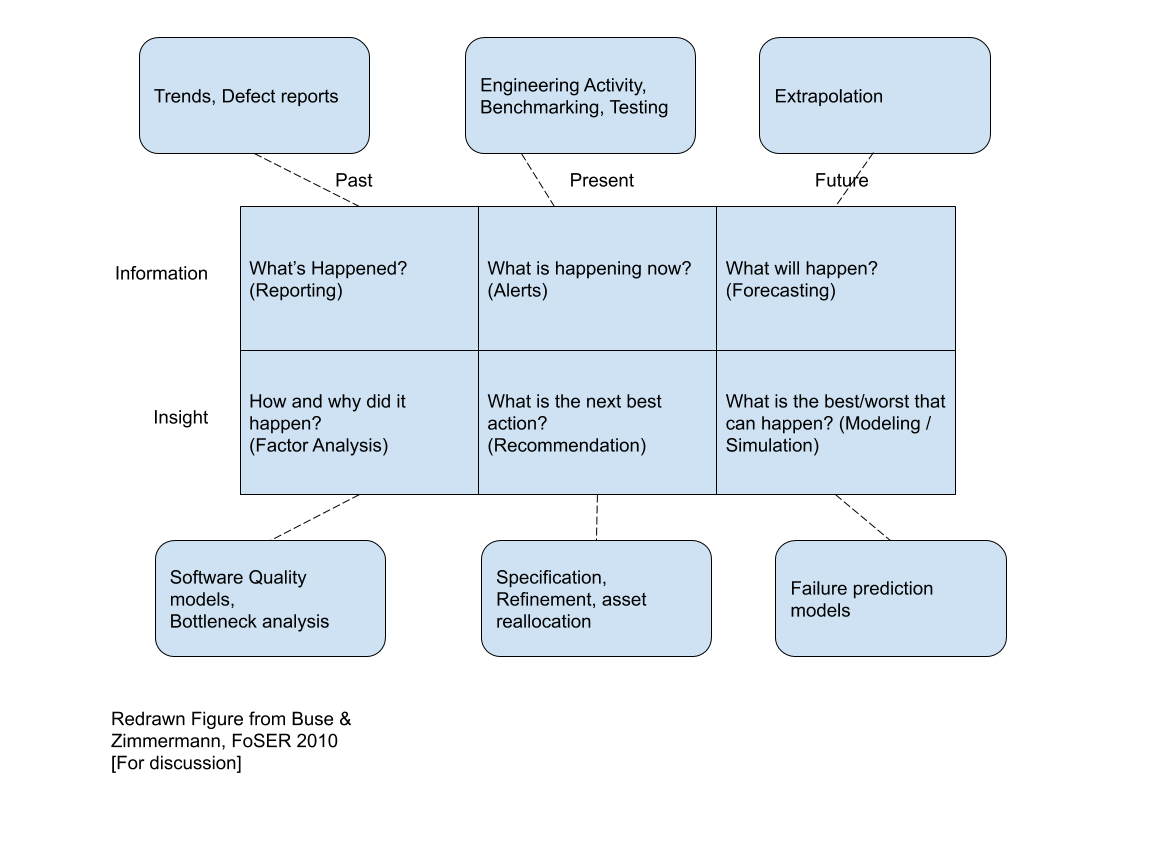
\includegraphics[width=\textwidth]{images/Buse_and_Zimmermann_2010_figure.png}
    \caption{Software Analytics: Buse and Zimmermann}
    \label{fig:buse_and_zimmermann_2010_figure}
\end{figure}

\subsection{Crashlytics and Google Firebase}
Google has acquired several major products related to runtime information gathering, including Crashlytics, Fabric\footnote{\url{https://get.fabric.io/}} and Firebase; as well as an automated testing service that seems to have been woven into the overall Google Firebase offering\footnote{Fabric will be retired on 31st March 2020 according to \\ \url{https://fabric.io/blog/updates-to-migration-roadmap-and-timeline}}. 

As table \ref{tab:appbrain_libraries_installed} shows these libraries are popular; and in particular Firebase is incorporated in over 54\% of Android apps (in >420,000 apps\footnote{\url{https://www.appbrain.com/stats/libraries/details/firebase/firebase}}) and in use in over 74\%!
% TODO add refs and check my claims are true. Did Google also acquire the germs of the device farm?

\begin{table}[]
    \centering
    \begin{tabular}{r|r|l}
    Apps &Installs &library \\
    12.25\% &20.01\%  & Fabric \\
    54.13\% &74.46\%  & Firebase\\
    14.33\% &25.24\%  & Crashlytics
    \end{tabular}
    \caption{Market penetration of libraries; AppBrain 19 June 2019}
    \label{tab:appbrain_libraries_installed}
\end{table}

\section{Quality Improvement}
Some definitions and perceptions of quality and quality improvement.
\begin{itemize}
    \item Gerry Weinberg
    \item ISO
\end{itemize}

\subsection{Quality of Experience (QoE)}
\begin{itemize}
    \item How about Quality of User Experience, or even Quality of Perceived User Experience? to measure / assess user's satisfaction with using an app.
    \item QoE generally used in telecoms, some mention for video downloading in mobile apps (TODO add ref)
    \item Compare with ISO 9126 etc. and Quality in Use?
\end{itemize}

\section{Many routes to better software}

\begin{itemize}
    \item Routes that involve testing software (many and various forms of testing ranging from fully automated to observation-based). For observations c.f. various usability testing techniques e.g. talk-aloud protocol. Automated testing includes those written by the development team.
    \item Using code quality tools (could be integrated into the IDE and/or standalone)
\end{itemize}
\subsection{First among equals?}